\documentclass[a4paper,UTF8]{ctexart}

\usepackage{amsmath, amsthm, amssymb, amsfonts, hyperref, mathrsfs}%美国数学学会的包+?
\usepackage{geometry} %控制界面
\usepackage{bookmark}
\usepackage{fancyhdr} % header & footer
\usepackage{appendix} % 附录
\usepackage{tikz} %作图
\usepackage{graphicx} %插入图片的宏包
\usepackage{float} %设置图片浮动位置的宏包
%\usepackage{subfigure} %插入多图时用子图显示的宏包
\usepackage{listings} %引用代码
\usepackage{physics,mathtools} %物理数学工具
\usepackage{comment}
\usepackage{framed}
\usepackage{caption}
\usepackage{subcaption}
\geometry{top=2.5cm,bottom=2.5cm,left=2.5cm,right=2.5cm} % 布局要求
\pagestyle{fancy} % fancy分格
\fancyhf{} % 清除所有页眉页脚
\renewcommand\headrulewidth{0.6pt}
\renewcommand\footrulewidth{0.6pt}
% font
\setCJKmainfont{Noto Serif CJK SC}[BoldFont={Noto Serif CJK SC Bold}, ItalicFont=]
\lhead{何金铭 PB21020660$\mid$座位号:1}
\cfoot{高阶涡旋光束的产生与检测预习报告}
\rhead{\thepage}
\lfoot{2024.4.17}
\rfoot{USTC}
%\bibliographystyle{plain} % 引用样式
\everymath{\displaystyle} % display
%============================================================

\begin{document}

\begin{center}
    \textbf{\Large 高阶涡旋光束的产生与检测预习报告}
    \par \text{\large 何金铭 PB21020660}
\end{center}

\section{实验目的}

本实验将利用q波片分别产生角向偏振光束、径向偏振光束和高阶矢量光束,并检测其特殊的偏振分布状态;利用螺旋相位片分别产生一阶和高阶相位涡旋光束,并检测其特殊的相位分布特性。

\section{实验简介}

涡旋光束是一种横向光强分布为“甜甜圈”形状的特殊光场。因为涡旋光束中心有奇异点,所以其中心光强为零。常说的涡旋光束主要有两种:

\begin{enumerate}
    \item 偏振涡旋光束(矢量光束):矢量光束的电场振动方向在光束横截面上具有中心轴对称性,光束的波振面呈漩涡状,中心呈现偏振奇异性。
    \item 第二种是相位涡旋光束(轨道角动量光束):相位涡旋光束具有螺旋形的波前,中心呈现相位奇异性。
\end{enumerate}

\section{实验原理}

\subsection{涡旋光束}

相位涡旋光束是光波的相位或波前呈螺旋形分布的光束,不同阶数的相位涡旋光束在横截面上的相位分布如下图所示。

\begin{figure}[H]
    \centering
    \begin{minipage}[b]{0.9\textwidth}
        \centering
        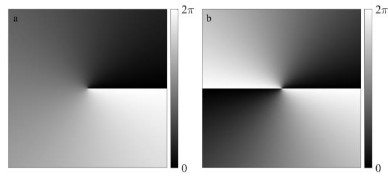
\includegraphics[width=0.6\textwidth]{./fig2.jpg}
        \caption{(a)一阶螺旋相位分布;(b)二阶螺旋相位分布}
    \end{minipage}
\end{figure}

\begin{figure}[H]
    \centering
    \begin{minipage}[b]{0.9\textwidth}
        \centering
        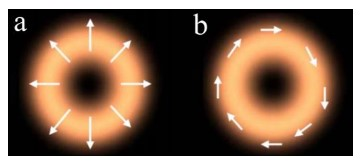
\includegraphics[width=0.6\textwidth]{./fig3.jpg}
        \caption{(a)径向偏振光;(b)角向偏振光}
    \end{minipage}
\end{figure}

矢量光束是偏振态在光束横截面上按照一定规律分布的光束,本实验主要考虑横截面偏振态呈涡旋分布的偏振涡旋光束。其中,一阶矢量光束也称为柱矢量光束,是一种特殊偏振态分布的矢量光束,其特点是偏振态在垂直于波矢方向的
横截面上呈轴对称特性分布。柱矢量光束主要包括径向偏振光和角向偏振光,径向偏振光的偏振方向呈辐射状分布,角向偏振光为环绕状分布,如图2所示。通常将偏振或者相位阶次大于1的涡旋光束称为高阶涡旋光束。

\subsection{基本器件}

\subsubsection{q波片}

\begin{figure}[H]
    \centering
    \begin{minipage}[b]{0.9\textwidth}
        \centering
        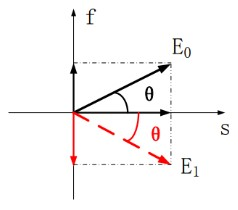
\includegraphics[width=0.5\textwidth]{./fig4.jpg}
        \caption{半波片旋转偏振方向原理}
    \end{minipage}
\end{figure}

q波片是一种由向列相液晶制成的可实现光束的自旋角动量与轨道角动量交换的偏振调制器,
其通过控制液晶分子主轴在横截面上的不均匀分布,在横截面每一点上形成一个局部半波片
(半波片旋转偏振方向原理如上图所示)。
若入射光束为线偏振光,则输出光场为具有各向异性偏振分布的矢量光束。

\begin{figure}[H]
    \centering
    \begin{minipage}[b]{0.9\textwidth}
        \centering
        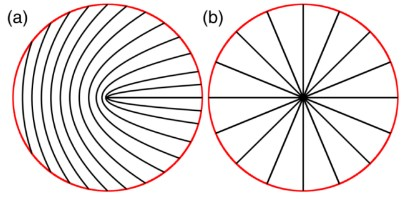
\includegraphics[width=0.6\textwidth]{./fig5.jpg}
        \caption{(a)一阶q波片;(b)二阶q波片(实线为主轴排列)}
    \end{minipage}
\end{figure}

极坐标系下q波片的液晶主轴在其横截面上的分布规律为:

\begin{equation}\alpha(r,\varphi)=q\varphi+\alpha_0\end{equation}

$q=m\times 0.5(m=1,2,3,\dots)$, m\text{为波片的阶数;} $\alpha_0$\text{为 }$\varphi=0$\text{时的初始主轴方向。}

\subsubsection{螺旋相位片}

\begin{figure}[H]
    \centering
    \begin{minipage}[b]{0.9\textwidth}
        \centering
        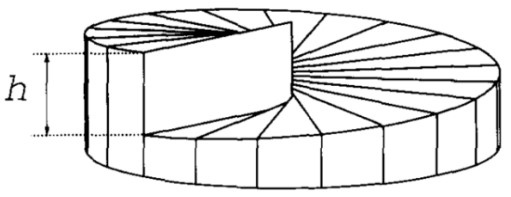
\includegraphics[width=0.6\textwidth]{./fig6.jpg}
        \caption{螺旋相位片结构示意图}
    \end{minipage}
\end{figure}

螺旋相位片(Spiral Phase Plate, SPP)一般是由对入射光透明的材料制成,其厚度在角向上并不均匀,使得当平面波入射时,可在不同的角向坐标处引入不同的相位延迟,进而将平面波前调制成螺旋波前。

\section{实验内容}

实验装置示意图如下:

\begin{figure}[H]
    \centering
    \begin{minipage}[b]{0.9\textwidth}
        \centering
        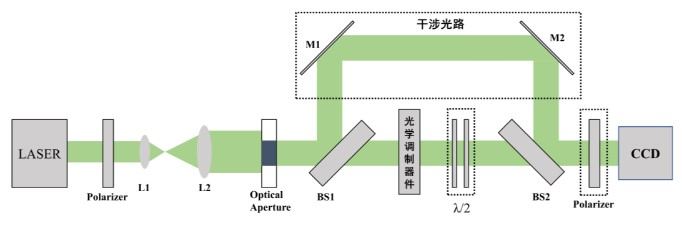
\includegraphics[width=0.9\textwidth]{./fig1.jpg}
        \caption{实验装置示意图}
    \end{minipage}
\end{figure}

利用级联片、偏振片、二阶q波片、一阶和二阶螺旋相位器、更高阶的光学调制器件来完成实验。

具体实验步骤如下:

\begin{enumerate}
    \item 调整光路,在未加级联片的情况下,使之输出径向偏振光,并利用偏振片检测其偏振状态,记录实验图像。
    \item 加入级联片,使之输出角向偏振光束,并利用偏振片检测其偏振状态,记录实验图像。
    \item 更换二阶q波片输出二阶矢量光束,并利用偏振片检测其偏振状态,记录实验图像。
    \item 使用一阶和二阶螺旋相位片,输出一阶和二阶相位涡旋光束,并搭建干涉光路检查其相位特性,记录实验图像。
    \item 更换更高阶的光学调制器件,产生并检测更高阶的矢量光束和相位涡旋光束,实验记录图像。
\end{enumerate}

\end{document}